\documentclass[10pt]{article}
\usepackage[preprint]{tmlr}
\usepackage{microtype}
\usepackage{amsmath,amssymb,amsthm}
\usepackage{booktabs}
\usepackage{tabularx}
\usepackage{array}
\usepackage{enumitem}
\usepackage[section]{placeins}
\usepackage{xcolor}
\usepackage{pgfplots}
\pgfplotsset{compat=1.18}
\usepackage{xurl}
\usepackage[hidelinks]{hyperref}

\newtheorem{proposition}{Proposition}
\newtheorem{definition}{Definition}
\newtheorem{remark}{Remark}

\newcommand{\Gr}{\mathrm{Gr}}
\newcommand{\NF}{\operatorname{NF}}
\newcommand{\Q}{\mathbb{Q}}
\newcommand{\R}{\mathbb{R}}

\title{Exact Grading of Proposed Polynomial Invariants}

\author{Tesfay Zemuy Gebrekidan\\
  Independent Researcher}

\InputIfFileExists{docs/tables_generated.tex}{}{\InputIfFileExists{tables_generated.tex}{}{\PackageError{paper}{Generate the result tables as described in the accompanying README}{}}}
\InputIfFileExists{docs/claims_generated.tex}{}{\newcommand{\nLLM}{1200}
\newcommand{\nBaseline}{150}
\newcommand{\nPrimary}{1350}
\newcommand{\nExact}{853}
\newcommand{\nNonReference}{36}
\newcommand{\nFirstValid}{889}
\newcommand{\nAllValid}{889}
\newcommand{\nGapCells}{13}
\newcommand{\nZeroGapCells}{47}
\newcommand{\minGap}{5}
\newcommand{\maxGap}{30}
\newcommand{\medianGap}{0}
\newcommand{\medianPositiveGap}{10}
\newcommand{\nMulti}{0}
\newcommand{\nAllLoss}{0}
\newcommand{\nBestGain}{0}
\newcommand{\nUnparseable}{30}
\newcommand{\nDecimal}{8}
\newcommand{\nCriterionTaskOnly}{110}
\newcommand{\nCriterionOnly}{0}
\newcommand{\nFit}{141}
\newcommand{\nFitLow}{0}
\newcommand{\nFitMid}{19}
\newcommand{\nLegacyLow}{0}
\newcommand{\nLegacyMid}{22}
\newcommand{\nKepler}{238}
\newcommand{\nKeplerEnergy}{133}
\newcommand{\nKeplerAngular}{104}
\newcommand{\nAcrobot}{270}
\newcommand{\nAcrobotExact}{14}
\newcommand{\nCASLiteral}{1198}
\newcommand{\nCASReconstructed}{29}
\newcommand{\nCASNonalgebraic}{152}
}
\begin{document}
\maketitle
\begin{abstract}
A polynomial proposal can satisfy a conservation task without matching a reference, or fit observations without being exactly conserved. We present a source-agnostic grading protocol over $\mathbb{Q}$ that separates literal task validity, reference recovery, rational reconstruction and generating-set completeness. Its empirical audit uses \nLLM{} language-model responses from three deployments and \nBaseline{} sparse numerical-baseline outputs on five system families and their variants. For the language models, literal validity credits \nFirstValid{} answers versus \nExact{} reference recoveries. The \nNonReference{} additional valid answers are all polynomial functions of known references, such as $E^2$ when $E$ is conserved: they satisfy the task without supplying independent invariants. Scores differ by \minGap{}--\maxGap{} percentage points in \nGapCells{} of 60 cells; the median gap is zero. For the sparse baseline, a tolerance-based comparator credits 20 reference recoveries versus 8 under literal coefficient interpretation. A separate 150-output rational multi-output baseline illustrates the distinction between valid individual constraints and complete generating sets. The protocol grades proposals regardless of their origin; establishing discovery rather than recall requires separate task-design evidence. Cached outputs and a Singular cross-check support offline regrading.
\end{abstract}

\noindent\textbf{Keywords:} exact verification, evaluation protocols, polynomial invariants, conservation laws, Gr\"obner bases.

\section{Introduction}

Polynomial proposals arise from language models, numerical regression and symbolic procedures.\footnote{OpenAI's Codex assisted with manuscript editing, code changes and consistency checks. The author is responsible for the claims and results.} Whatever their source, an evaluator must decide whether to credit a reference match, an exact conservation identity, an approximate fit or a complete set of constraints. These criteria answer different questions. On identical stored LLM responses, we find that reference recovery and literal task validity differ by up to \maxGap{} percentage points per cell, although most cells have no gap. For the sparse numerical baseline, a tolerance-based coefficient policy credits 20 reference recoveries while literal interpretation credits 8. The contribution is an exact grading protocol and an audit of what these choices change.

For example, if $E=w_1^2+2w_2^2+3w_3^2$ is conserved, both $E$ and $E^2$ answer a conservation task, but only $E$ is an affine reference recovery. The polynomial $E+10^{-10}w_2^2$ fails exact conservation, although rational reconstruction can recover $E$. These examples motivate separate reporting of literal task validity, reference recovery and reconstruction-dependent validity.

We implement this distinction for two tasks: recovering a generating set for an implicit constraint ideal, and finding a nonconstant polynomial conserved by supplied dynamics. Ideal membership and equality test the first; a Lie derivative reduced modulo known constraints tests the second. The checks operate over $\Q$ on a declared regular domain and reuse the established \texttt{algebraicRLtest} routines accompanying \citet{gebrekidan2026diagnosing}. Our protocol adds literal coefficient interpretation, separate reconstruction outcomes, explicit handling of trivial and incomplete answers, and a numerical diagnostic that removes additive constants and known constraints.

The audit uses \nLLM{} LLM responses and \nBaseline{} sparse numerical-baseline outputs, with a further 150-output rational multi-output baseline. Scoring rules receive the same expressions from a fixed five-family suite. Exact definitions, saved prompts and responses, and a Singular cross-check make the measurements regradable. These outputs supply test material for the protocol; correct answers do not establish discovery or derivation independently of recall.

\section{Related Work}

\paragraph{Discovery benchmarks.} LLM-SRBench \citep{shojaee2025llmsrbench} and NewtonBench \citep{newtonbench2026} use LLM judges for structural equation equivalence, setting aside parameter or physical-constant values and reporting numerical fidelity separately. DiscoveryBench \citep{majumder2025discoverybench} evaluates natural-language hypotheses. SRBench \citep{lacava2021srbench} simplifies expression differences or ratios; SRSD \citep{matsubara2024srsd} also measures expression-tree edit distance. ERBench \citep{kahlmeyer2026erbench} distinguishes equation recovery from predictive fit and uses numerical equivalence checks after comparing them with symbolic checks. These benchmarks already distinguish several evaluation objectives. Here the target is a conservation identity or an entire constraint ideal, and we measure disagreements between literal validity, reference recovery and reconstruction on identical outputs. We do not re-evaluate those benchmarks or compare verifier accuracy on their tasks.

\paragraph{Conservation-law discovery and verification.} The kernel method of \citet{mebratie2025conservation} validates candidates numerically and describes refinement using the symbolic conservation equation. \citet{hybridode2025} tests differentiated candidates against a learned vector field; NGCG \citep{ngcg2026} uses trajectory constancy and a diversity filter. Exact methods are also established: \citet{desoeuvres2024polynomial} compute polynomial conservation laws using comprehensive Gr\"obner systems and syzygies, while FISolver \citep{fisolver2026} symbolically verifies LLM-generated first integrals of two-dimensional ODEs. We use supplied reference dynamics and constraint ideals to audit literal polynomial answers. Differential-radical invariants \citep{ghorbal2014differential} address invariance of algebraic sets, which differs from constancy of an observable along every trajectory.

\paragraph{Independent structure and numerical synthesis.} AI Poincar\'e \citep{liu2021poincare} discovers conservation structure from trajectories; AI Poincar\'e 2.0 \citep{liu2022poincare} explicitly addresses functional independence. Our reference-product checks explain dependencies without testing independence. SINDy \citep{brunton2016sindy} identifies sparse dynamics, implicit-SINDy \citep{mangan2016implicit} searches feature nullspaces, and SINDy-PI \citep{kaheman2020sindypi} uses parallel sparse regressions and model selection. These motivate our custom numerical procedures, built with PySINDy components \citep{kaptanoglu2022pysindy}; neither procedure is an evaluation of a standard PySINDy estimator.

\section{Method: exact grading}\label{sec:grader}

\subsection{Algebraic task criteria}

Each task declares variables $x$, a reference ideal $I\subseteq\Q[x]$ and, for conservation tasks, rational dynamics and reference conserved polynomials. Write $\NF_I$ for reduction modulo a reduced Gr\"obner basis of $I$. The two tasks are to generate the entire reference ideal or to return a nonconstant conserved polynomial modulo the known constraints.

For vanishing constraints, the grader checks membership in the reference ideal by normal-form reduction and equality of ideals by mutual reduction. Reduced Gr\"obner bases are computed over $\Q$ in \texttt{grevlex} order \citep{cox2015ideals}. Ideal membership, equality and affine-span membership in the quotient ring are independent of term order when candidates and references share the normal-form map.

Conserved quantities form a subalgebra and generally do not form an ideal \citep{gebrekidan2026diagnosing}. For dynamics $\dot x=f(x)/d(x)$ with polynomial numerator $f$, the test is $\NF_I(\nabla Q\cdot f)=0$. Provided the field preserves the constraints, this certifies conservation along trajectories in $V_\R(I)\cap\{d\ne0\}$. A converse requires $I$ to capture the polynomial identities of that domain. Appendix~\ref{app:domain} explains this distinction and checks denominator saturation for the benchmark.

A conserved polynomial is nontrivial when it is nonconstant in the supplied quotient ring. Affine combinations of reference invariants count as reference recovery; other nontrivial conserved polynomials are task-valid non-reference answers. Products of references of degree at most two are tested to explain dependencies (Appendix~\ref{app:verdicts}). Table~\ref{tab:decisions} summarises the decisions; refusals, empty completions, parsing failures and unavailable computations remain distinct outcomes.

\begin{table}[!htbp]
\centering\small
\begin{tabularx}{\textwidth}{@{}p{2.5cm}XX@{}}
\toprule
Decision & Conserved-quantity task & Generating-set task \\
\midrule
Literal validity & Zero Lie remainder and nonconstant in the quotient & Every polynomial is in the ideal and the set generates it \\
Reference recovery & Additionally lies in the affine reference span & Coincides with literal task validity \\
Partial or trivial & Constant in the quotient is trivial & Membership without equality is incomplete \\
Reconstruction & Record recovered sub-verdict separately; exclude from literal validity & Distinguish reconstructed complete and incomplete sets \\
\bottomrule
\end{tabularx}
\caption{Core grading decisions. Refusals, empty responses, parsing failures and unavailable computations are recorded separately.}
\label{tab:decisions}
\end{table}

\paragraph{Numerical proximity.} Algebraic failures receive a separate residual or drift diagnostic, with threshold $10^{-3}$. For conservation, we evaluate the quotient representative after removing its constant coefficient, so adding a constant or a known constraint does not change the algebraic diagnostic. The score is scale invariant but can depend on coordinates and term order. It never overrides an exact verdict. Appendix~\ref{app:sensitivity} gives the normalisation, exceptional cases and sensitivity comparison.

\subsection{Scoring and output policies}

The primary scores are \emph{reference recovery} and \emph{literal task validity}. Reference recovery means affine-span recovery for conservation tasks and ideal equality for curve tasks; pooled counts include both. Literal validity additionally credits non-reference conserved polynomials. The conservation task asks for one conserved polynomial nonconstant in the quotient, so $E^2$ is task-valid. The curve task asks for a generating set, so an incomplete set fails both scores. Appendix~\ref{app:verdicts} maps these outcomes to archive labels; Appendix~\ref{app:scoring} examines a constructed permissive score that accepts reconstructed, trivial and incomplete answers.

\paragraph{Multi-polynomial answers.} Conservation answers are scored by their first polynomial; all returned polynomials are also graded at $D=1000$ and archived. A first-member rule depends on ordering, an any-member rule can reward longer lists, and an all-members rule rejects a list containing a spurious answer. For conservation, ``all valid'' requires every returned expression to be nontrivially conserved, excluding constants and constraint-only expressions. Curve answers are graded jointly as generating sets; their first/any/all columns all use this joint verdict. Section~\ref{sec:results} compares these policies on the stored outputs.

\subsection{Literal coefficients and rational reconstruction}

A restricted arithmetic parser accepts declared variables, rational literals, parentheses and polynomial operations without evaluating Python code. Integers, fractions, decimals and scientific notation are interpreted exactly before expansion: $0.1+0.2=0.3$, while $2.0000000001\ne2$. Irrational coefficients and non-polynomial expressions are rejected. Literal validity has no coefficient tolerance; exact decimal multiples of an invariant remain valid.

The reconstruction diagnostic replaces decimal tokens by nearest rationals with denominator at most $D\in\{10,100,1000\}$; fractions written with integers are unchanged. A literal algebraic failure repaired to a reference, a valid non-reference polynomial or an incomplete generating set is recorded as reconstruction-dependent, with both verdicts stored. Already conserved candidates and sets whose members all lie in the reference ideal retain their literal verdicts, as do unavailable computations. The main diagnostic uses $D=1000$; a record is \emph{reconstruction-sensitive} if its outer or reconstructed verdict changes across caps, including incomplete-to-complete transitions beneath the same outer label. Literal validity is independent of $D$.

The caps probe increasingly complex small-denominator repairs. They do not estimate measurement precision or statistical confidence. Reconstruction can erase a genuine small term or repair an accidental finite-sample fit. Exact rechecking certifies the repaired polynomial against the target; it does not establish coefficient identifiability from the observations.

\paragraph{Validation.} Controls and regressions check rewritten references, rational perturbations, triviality, coefficient parsing, reconstruction, prompt leakage and multi-polynomial answers. Separate checks verify tangency to constraints, compare symbolic derivatives with numerical trajectories, and cross-check the Acrobot derivation. Commands are supplied in the archive.

\section{Experimental setup}\label{sec:protocol}

The \emph{primary dataset} contains \nLLM{} LLM responses and \nBaseline{} sparse numerical-baseline outputs, 1,350 records in total. A separate 150-output rational multi-output baseline tests coefficient recovery and output-set policies. These proposers supply different kinds of answers to audit; their success rates do not identify how the LLMs produced their answers.

\subsection{Benchmark and input conditions}\label{sec:benchmark}

Each system supplies variables, a generating set of its vanishing ideal (possibly empty), a polynomial vector-field numerator with its common denominator, and reference invariants, all exact over $\Q$. Table~\ref{tab:systems} lists the systems. Each system has a canonical form and a variant with changed parameters or coordinates, referred to as its perturbed twin. The Acrobot energy is cross-checked symbolically against the implementation accompanying \citet{gebrekidan2026diagnosing}; numerical derivatives are also compared with its reference dynamics in the independent test suite.

\begin{table}[!htbp]
\centering
\small
\renewcommand{\arraystretch}{1.15}
\begin{tabularx}{\textwidth}{@{}>{\raggedright\arraybackslash}p{2.5cm}
                               >{\raggedright\arraybackslash}p{2.9cm}
                               >{\raggedright\arraybackslash}p{1.7cm}
                               >{\raggedright\arraybackslash}X@{}}
\toprule
System & Variables & Task type & Reference object \\
\midrule
Twisted cubic & $x,y,z$ & vanishing ideal & $I=(y-x^{2},\,z-x^{3})$; reduced Gr\"obner basis has three elements \\
Free rigid body ($I=1,2,3$) & $w_{1},w_{2},w_{3}$ & conserved quantity & energy and squared angular momentum \\
Planar Kepler, lifted & $x,y,v_{x},v_{y},u=1/r$ & conserved quantity & energy, angular momentum, Laplace--Runge--Lenz components; constraint $u^{2}(x^{2}+y^{2})=1$ \\
Moiety network ($A+B\leftrightarrow C$, $C\to D$) & $A,B,C,D$ & conserved quantity & $A-B$ and $A+C+D$ (linear) \\
Acrobot (book model, passive) & $c_{1},s_{1},c_{2},s_{2},w_{1},w_{2}$ & conserved quantity & energy, degree 3; constraints $c_{i}^{2}+s_{i}^{2}=1$ \\
\midrule
Perturbed twins (5) & renamed & as canonical & twisted cubic $(t,2t^{2}-1,t^{3}+t)$; rigid body $I=(3,5,11)$; Kepler $\mu=3/2$; moiety $2A+B\leftrightarrow C$; Acrobot with $m_{2}=13/10$, $l_{1}=6/5$, $l_{c2}=3/5$, $I_{2}=3/2$ \\
\bottomrule
\end{tabularx}
\caption{Benchmark systems (canonical rows) and perturbed twins. The perturbed Acrobot energy and dynamics are derived symbolically from the parameters. With default parameters, the derived energy matches the reference polynomial exactly, and the derived vector field agrees with the reference dynamics at 100 random states to within $10^{-9}$.}
\label{tab:systems}
\end{table}

We evaluate canonical systems and their twins under two input conditions. Condition A supplies equations of motion or the curve parametrisation. Condition B supplies sampled states and a description specifying the parameters and mechanism; only the twisted-cubic description is parameter-free. No observational noise is added ($\sigma=0$); sampled coordinates are rounded for display in the prompts.

Prompts request a JSON object with a \texttt{polynomials} list and a \texttt{refuse} flag. Conservation prompts ask for exactly one nonconstant conserved polynomial; curve prompts ask for a generating set. Stored prompt strings, including system descriptions and known constraints, are included in the release.

Twins change parameters and rename variables. The rigid-body, Kepler and Acrobot invariants remain parametric textbook formulas, so formula recall can suffice. The moiety twin changes reaction stoichiometry, and the curve twin applies an invertible polynomial coordinate transformation. These variants probe parameter and notation generalisation; they do not rule out formula recall. Only the twisted cubic and its coordinate twin exercise generating-set completeness.

\paragraph{Curve-task contract.} Both curve conditions request generators for the ideal of the entire underlying parametrised curve. Condition B identifies decimals as rounded observations and states that finite samples do not determine an unrestricted curve uniquely. A response must propose a candidate curve or refuse; the grader tests that candidate against the underlying-curve ideal, rather than the ideal of the displayed points.

\subsection{LLM deployments and sampling}

The LLM experiment contains 400 responses per deployment: ten systems, two conditions (A and B), and 20 slots per cell, for \nLLM{} responses. Two providers serve the same named gpt-oss model; the third serves Gemini. The recorded deployments and settings are:
\begin{enumerate}[label=(\roman*),leftmargin=*]
\item Groq \texttt{openai/gpt-oss-120b} \citep{openai-gpt-oss}: temperature 1, reasoning effort \texttt{medium}, collection 29 October--4 November 2026.
\item Cerebras \texttt{gpt-oss-120b}: temperature 1, reasoning effort \texttt{medium}, collection 29--30 October 2026.
\item Google AI Studio \texttt{gemini-3.5-flash-lite}: thinking level \texttt{medium}, temperature omitted (the effective provider default was not measured), collection 29--30 October 2026.
\end{enumerate}
All deployments receive a 4,000-token completion cap, including reasoning where the API counts it. Effective reasoning compute and provider defaults can differ. No tools are supplied or executed. The frozen plan lists exact prompts and omitted parameters; raw records contain usage, finish status, returned model identifier and fingerprint where supplied. The same shuffled slot order and sampled data are shared across providers.

\paragraph{Sampled inputs.} Condition B provides 25 sampled states from one trajectory of duration 3 for dynamical systems, or 25 points on the parametrised curve. Trajectories are integrated using DOP853 with relative and absolute tolerances $10^{-12}$ and $10^{-13}$. The LLM prompts supply known algebraic constraints, whereas the numerical baselines do not receive them or deflate their span, so they can rediscover constraints classified as trivial.

\subsection{Numerical proposal baselines}\label{sec:numerical-baselines}

Two diagnostic numerical procedures each produce 150 outputs (15 seeds per system). Both use sampled states without the LLM descriptions or known constraints and share a PySINDy polynomial library and fourth-order finite differences. Neither receives the exact field or reference polynomials during synthesis. The data are generated by integrating the reference dynamics. These collections are labelled condition B in the archive, but their information and sampling budgets differ from the LLM condition B.

\paragraph{Sparse single-output procedure.} This implicit-SINDy-style search \citep{mangan2016implicit} uses six trajectories of duration 2 with 2,000 states each, or 600 curve points. Library degree is 3 for the curve, Kepler and Acrobot, and 2 otherwise; five derivative samples are discarded at each endpoint. A column-normalised smallest-singular-vector search thresholds at $0.05$ of the largest coefficient and refits for up to eight iterations. After mapping back to monomial coordinates, terms of magnitude at most $10^{-8}$ are omitted and coefficients are printed to 12 significant digits. Both curve ideals have height two, so a single polynomial cannot generate them. Grading diagnostics use fixed seed-0 samples: six trajectories of duration 4 with 400 states each, or 2,000 curve points. These can overlap discovery samples; the diagnostic is not a held-out generalisation test.

\paragraph{Rational multi-output procedure.} With the same sampling budgets and library degrees, a column-normalised SVD estimates a nullspace using relative threshold $10^{-7}$. Pivoted QR selects coordinates for an identity-block basis, reducing dependence on arbitrary SVD basis mixtures. Each coefficient is approximated by a rational with denominator at most 1000, and all basis polynomials are emitted. Rational recovery occurs during discovery; the grader checks the emitted fractions literally.

\subsection{Response accounting and uncertainty}

\paragraph{Transport accounting and returned answers.} Cerebras and Gemini each delivered 400 responses; Groq initially delivered 379. After three failed transport attempts per missing slot, a follow-up recovered all 21 using byte-identical prompts and unchanged generation settings. Original failures, retry settings and follow-up attempts are archived. Final cell denominators are 20. Empty, refused, invalid and truncated answers were never resampled. Completion limits stopped 38 Groq, 42 Cerebras and 26 Gemini responses.

\paragraph{Scope of comparisons.} We report Wilson 95\% intervals for each of the 60 LLM cells. They use a binomial sampling approximation: A repeats the same prompt, while B varies the sampled observations across slots. They do not account for service drift, dependence between requests, or generalisation across families. Provider defaults, reasoning compute and collection times are not controlled to be equal. All grading-policy comparisons use identical stored answers; the study does not establish a capability ranking between providers or discovery procedures.

\section{Results}\label{sec:results}

We report score disagreements on identical stored outputs, separating reference recovery, coefficient policies and output-set policies. Appendix~\ref{app:deployments} gives complete deployment results.

\subsection{Reference recovery versus task validity}

\begin{figure}[t]
\centering
\InputIfFileExists{docs/figure_metric_gap.tex}{}{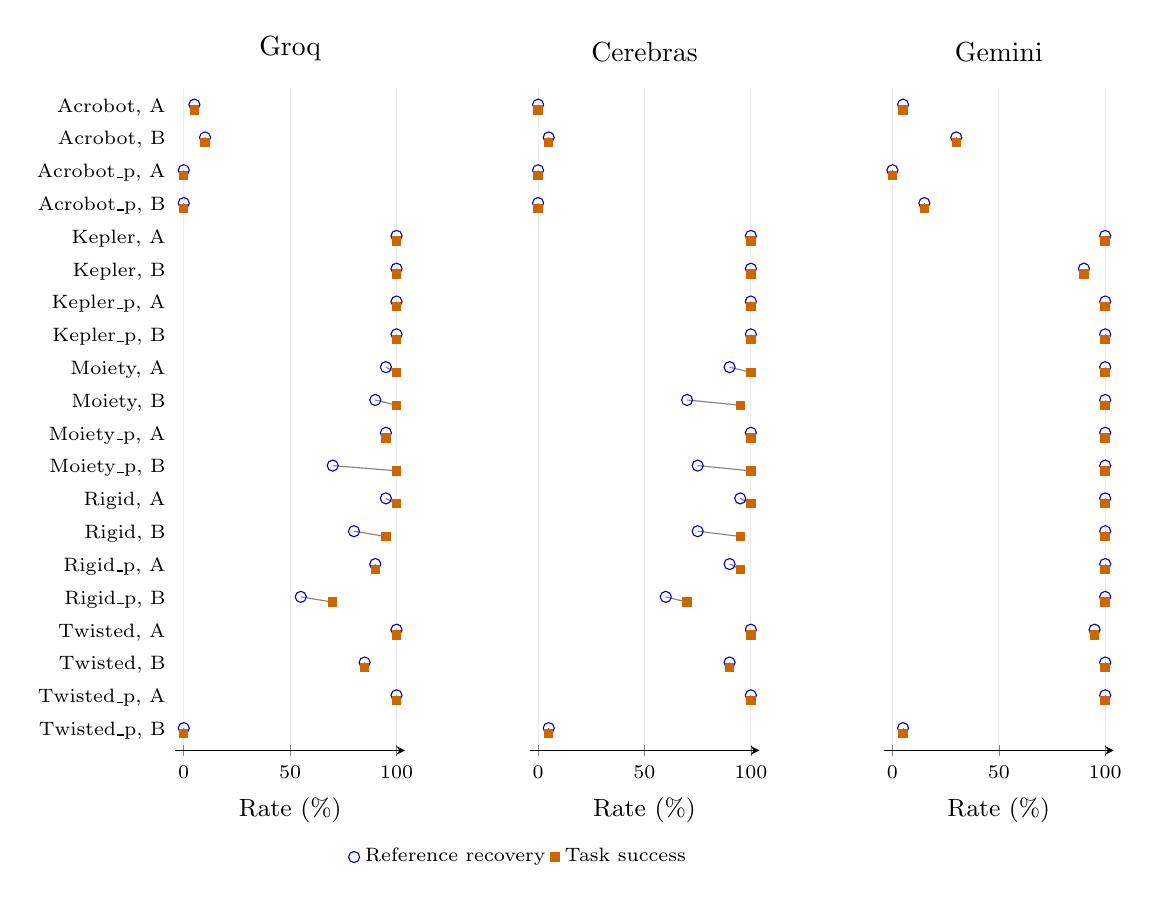
\begin{tikzpicture}
\begin{axis}[at={(0.0cm,0)},anchor=west,width=4.5cm,height=10cm,xmin=-4,xmax=104,ymin=0.4,ymax=20.6,xtick={0,50,100},xlabel={Rate (\%)},ytick={20,19,18,17,16,15,14,13,12,11,10,9,8,7,6,5,4,3,2,1},yticklabels={{Acrobot, A},{Acrobot, B},{Acrobot\_p, A},{Acrobot\_p, B},{Kepler, A},{Kepler, B},{Kepler\_p, A},{Kepler\_p, B},{Moiety, A},{Moiety, B},{Moiety\_p, A},{Moiety\_p, B},{Rigid, A},{Rigid, B},{Rigid\_p, A},{Rigid\_p, B},{Twisted, A},{Twisted, B},{Twisted\_p, A},{Twisted\_p, B}},tick label style={font=\scriptsize},label style={font=\small},xmajorgrids=true,grid style={gray!15},axis y line*=left,axis x line=bottom,y axis line style={draw=none},ytick style={draw=none},title={Groq},legend style={font=\scriptsize,draw=none,at={(1.5,-0.13)},anchor=north,legend columns=2}]
\addplot[gray,thin,unbounded coords=jump] coordinates {(5,20.08) (5,19.92) (nan,nan) (10,19.08) (10,18.92) (nan,nan) (0,18.08) (0,17.92) (nan,nan) (0,17.08) (0,16.92) (nan,nan) (100,16.08) (100,15.92) (nan,nan) (100,15.08) (100,14.92) (nan,nan) (100,14.08) (100,13.92) (nan,nan) (100,13.08) (100,12.92) (nan,nan) (95,12.08) (100,11.92) (nan,nan) (90,11.08) (100,10.92) (nan,nan) (95,10.08) (95,9.92) (nan,nan) (70,9.08) (100,8.92) (nan,nan) (95,8.08) (100,7.92) (nan,nan) (80,7.08) (95,6.92) (nan,nan) (90,6.08) (90,5.92) (nan,nan) (55,5.08) (70,4.92) (nan,nan) (100,4.08) (100,3.92) (nan,nan) (85,3.08) (85,2.92) (nan,nan) (100,2.08) (100,1.92) (nan,nan) (0,1.08) (0,0.92) (nan,nan)};
\addplot[only marks,mark=o,blue!75!black] coordinates {(5,20.08) (10,19.08) (0,18.08) (0,17.08) (100,16.08) (100,15.08) (100,14.08) (100,13.08) (95,12.08) (90,11.08) (95,10.08) (70,9.08) (95,8.08) (80,7.08) (90,6.08) (55,5.08) (100,4.08) (85,3.08) (100,2.08) (0,1.08)};
\addplot[only marks,mark=square*,mark size=1.5pt,orange!80!black] coordinates {(5,19.92) (10,18.92) (0,17.92) (0,16.92) (100,15.92) (100,14.92) (100,13.92) (100,12.92) (100,11.92) (100,10.92) (95,9.92) (100,8.92) (100,7.92) (95,6.92) (90,5.92) (70,4.92) (100,3.92) (85,2.92) (100,1.92) (0,0.92)};
\legend{,Reference recovery,Task success}
\end{axis}
\begin{axis}[at={(4.5cm,0)},anchor=west,width=4.5cm,height=10cm,xmin=-4,xmax=104,ymin=0.4,ymax=20.6,xtick={0,50,100},xlabel={Rate (\%)},ytick={20,19,18,17,16,15,14,13,12,11,10,9,8,7,6,5,4,3,2,1},yticklabels={},tick label style={font=\scriptsize},label style={font=\small},xmajorgrids=true,grid style={gray!15},axis y line*=left,axis x line=bottom,y axis line style={draw=none},ytick style={draw=none},title={Cerebras},legend style={font=\scriptsize,draw=none,at={(1.5,-0.13)},anchor=north,legend columns=2}]
\addplot[gray,thin,unbounded coords=jump] coordinates {(0,20.08) (0,19.92) (nan,nan) (5,19.08) (5,18.92) (nan,nan) (0,18.08) (0,17.92) (nan,nan) (0,17.08) (0,16.92) (nan,nan) (100,16.08) (100,15.92) (nan,nan) (100,15.08) (100,14.92) (nan,nan) (100,14.08) (100,13.92) (nan,nan) (100,13.08) (100,12.92) (nan,nan) (90,12.08) (100,11.92) (nan,nan) (70,11.08) (95,10.92) (nan,nan) (100,10.08) (100,9.92) (nan,nan) (75,9.08) (100,8.92) (nan,nan) (95,8.08) (100,7.92) (nan,nan) (75,7.08) (95,6.92) (nan,nan) (90,6.08) (95,5.92) (nan,nan) (60,5.08) (70,4.92) (nan,nan) (100,4.08) (100,3.92) (nan,nan) (90,3.08) (90,2.92) (nan,nan) (100,2.08) (100,1.92) (nan,nan) (5,1.08) (5,0.92) (nan,nan)};
\addplot[only marks,mark=o,blue!75!black] coordinates {(0,20.08) (5,19.08) (0,18.08) (0,17.08) (100,16.08) (100,15.08) (100,14.08) (100,13.08) (90,12.08) (70,11.08) (100,10.08) (75,9.08) (95,8.08) (75,7.08) (90,6.08) (60,5.08) (100,4.08) (90,3.08) (100,2.08) (5,1.08)};
\addplot[only marks,mark=square*,mark size=1.5pt,orange!80!black] coordinates {(0,19.92) (5,18.92) (0,17.92) (0,16.92) (100,15.92) (100,14.92) (100,13.92) (100,12.92) (100,11.92) (95,10.92) (100,9.92) (100,8.92) (100,7.92) (95,6.92) (95,5.92) (70,4.92) (100,3.92) (90,2.92) (100,1.92) (5,0.92)};
\end{axis}
\begin{axis}[at={(9.0cm,0)},anchor=west,width=4.5cm,height=10cm,xmin=-4,xmax=104,ymin=0.4,ymax=20.6,xtick={0,50,100},xlabel={Rate (\%)},ytick={20,19,18,17,16,15,14,13,12,11,10,9,8,7,6,5,4,3,2,1},yticklabels={},tick label style={font=\scriptsize},label style={font=\small},xmajorgrids=true,grid style={gray!15},axis y line*=left,axis x line=bottom,y axis line style={draw=none},ytick style={draw=none},title={Gemini},legend style={font=\scriptsize,draw=none,at={(1.5,-0.13)},anchor=north,legend columns=2}]
\addplot[gray,thin,unbounded coords=jump] coordinates {(5,20.08) (5,19.92) (nan,nan) (30,19.08) (30,18.92) (nan,nan) (0,18.08) (0,17.92) (nan,nan) (15,17.08) (15,16.92) (nan,nan) (100,16.08) (100,15.92) (nan,nan) (90,15.08) (90,14.92) (nan,nan) (100,14.08) (100,13.92) (nan,nan) (100,13.08) (100,12.92) (nan,nan) (100,12.08) (100,11.92) (nan,nan) (100,11.08) (100,10.92) (nan,nan) (100,10.08) (100,9.92) (nan,nan) (100,9.08) (100,8.92) (nan,nan) (100,8.08) (100,7.92) (nan,nan) (100,7.08) (100,6.92) (nan,nan) (100,6.08) (100,5.92) (nan,nan) (100,5.08) (100,4.92) (nan,nan) (95,4.08) (95,3.92) (nan,nan) (100,3.08) (100,2.92) (nan,nan) (100,2.08) (100,1.92) (nan,nan) (5,1.08) (5,0.92) (nan,nan)};
\addplot[only marks,mark=o,blue!75!black] coordinates {(5,20.08) (30,19.08) (0,18.08) (15,17.08) (100,16.08) (90,15.08) (100,14.08) (100,13.08) (100,12.08) (100,11.08) (100,10.08) (100,9.08) (100,8.08) (100,7.08) (100,6.08) (100,5.08) (95,4.08) (100,3.08) (100,2.08) (5,1.08)};
\addplot[only marks,mark=square*,mark size=1.5pt,orange!80!black] coordinates {(5,19.92) (30,18.92) (0,17.92) (15,16.92) (100,15.92) (90,14.92) (100,13.92) (100,12.92) (100,11.92) (100,10.92) (100,9.92) (100,8.92) (100,7.92) (100,6.92) (100,5.92) (100,4.92) (95,3.92) (100,2.92) (100,1.92) (5,0.92)};
\end{axis}
\end{tikzpicture}
}
\caption{Reference recovery (open circles) and literal task validity (filled squares) for all 60 LLM cells. Rows show canonical systems and twins (p), under equations (A) or sampled states plus a description (B). Lines pair scores on identical outputs; markers are vertically offset. Curve scores assess the declared underlying-curve contract. Gaps occur in \nGapCells{} cells, all from the two gpt-oss deployments; \nZeroGapCells{} cells have zero gap. Cell denominators and Wilson intervals appear in Appendix~\ref{app:deployments}. }
\label{fig:metric-gap}
\end{figure}

\paragraph{Results for reference recovery and task validity.} Across \nLLM{} LLM responses, \nExact{} meet the reference-recovery criterion and \nNonReference{} more are literally task-valid, giving \nFirstValid{} task-valid answers. In the four canonical rigid-body cells from the two \texttt{gpt-oss} deployments, reference recovery is 75--95\% and task validity is 95--100\% ($n=20$ per cell); paired score gaps range from 5 to 20 percentage points. A polynomial quadratic in energy $E$ and squared angular momentum $L^2$ can satisfy conservation without lying in their affine span. Of the \nNonReference{} non-reference valid LLM answers, 35 are explained by reference products of degree at most two. The remaining Cerebras moiety answer is $(A-B)^3$, verified exactly as the cube of a listed reference. All 14 non-reference numerical-baseline answers are explained by degree-two reference products. Thus all non-reference answers in the primary LLM and sparse-baseline collection have explicit dependencies on the references.

\paragraph{Complete policy audit.} Across the 60 LLM cells, the reference-to-task-valid gap is nonzero in \nGapCells{}, ranges from \minGap{} to \maxGap{} points when nonzero, and has median \medianGap{} overall (\medianPositiveGap{} points among nonzero cells). All affected cells belong to the two gpt-oss deployments; Gemini has no such gap. Cerebras's canonical moiety B cell changes from 70\% reference recovery to 95\% task validity. Table~\ref{tab:policy-summary} reports the complete audit. The counts describe the fixed task mixture.

\begin{table}[!htbp]
\centering\small
\tabPolicySummary
\caption{LLM policy summary. Additional valid answers are task-valid but outside the affine reference span. Gap cells and maximum gaps compare these two scores across each deployment's 20 cells; gaps are percentage points. All returned responses remain in the denominators.}
\label{tab:policy-summary}
\end{table}

Appendix~\ref{app:criterion-transfer} compares these objectives with a transferred reference-equivalence criterion.

\subsection{Coefficient and output-set policies}

\paragraph{Results for literal coefficients and rational reconstruction.} The sparse baseline recovers an affine reference in 8 of 150 outputs, and a further 14 literal outputs are valid non-reference invariants. Twenty-nine answers are useful only after rational reconstruction: 24 recover a reference, 3 are valid non-reference and 2 are incomplete generating sets. None counts as literal task validity. The canonical twisted-cubic outputs are single relations, so a membership-only score would credit 15/15 while generating-set success is 0/15. The baseline's single-output interface makes generating-set success impossible on these tasks.

\begin{table}[!htbp]
\centering
\small
\setlength{\tabcolsep}{4pt}
\tabSINDy
\caption{Diagnostic sparse-nullspace baseline, condition B; counts out of 15 per row. Task-valid includes reference recovery and non-reference conserved quantities. Reconstructed answers are useful only after lossy reconstruction and are excluded from literal task validity; incomplete and trivial are literal verdicts. The five verdict columns are not disjoint because reference recovery is a subset of task-valid. The remaining outputs are algebraic failures (55 plausible and 25 implausible overall). Full verdict records and cap sensitivity are archived. Single-output twisted-cubic rows cannot satisfy the generating-set task by design.}
\label{tab:results-sindy}
\end{table}

\paragraph{First-polynomial rule.} The conservation prompt explicitly requests exactly one polynomial. No LLM conservation response returns multiple polynomials, so first-polynomial and all-returned-polynomials validity coincide: \nFirstValid{} task-valid LLM responses under either policy. Curve answers are assessed jointly under the contract in Section~\ref{sec:grader}.

\paragraph{Rational multi-output results.} The procedure in Section~\ref{sec:numerical-baselines} achieves literal generating-set success on all 30 twisted-cubic outputs, compared with zero for the archived single-output procedure. Across all 150 outputs, the first polynomial is task-valid in 134, at least one polynomial is task-valid in 135, and every polynomial is task-valid in 98 (Table~\ref{tab:rational-baseline}). Kepler's estimated nullity varies across seeds and Acrobot outputs can include known constraints or approximate directions. The pipeline solves the generating-set tasks, but some returned bases contain invalid or trivial members. Nullspace extraction, coefficient recovery and the output interface change together; their separate effects are not isolated. The singular values, estimated nullities, settings and raw outputs are stored.

\begin{table}[!htbp]
\centering\small
\tabRationalBaseline
\caption{Numerical baseline with rational recovery, 15 seeds per system. Conservation rows compare first, any and all returned nontrivial conserved polynomials. Generating-set rows assess the complete returned set under every column, rather than accepting a single member.}
\label{tab:rational-baseline}
\end{table}

\paragraph{Numerical proximity versus exact validity.} At $10^{-3}$, 84 sparse-baseline outputs fail literal algebraic checks despite small residual or drift, including all 29 reconstruction-dependent answers. No scored LLM algebraic failure lies below this threshold. Appendix~\ref{app:sensitivity} reports threshold sensitivity; Section~\ref{sec:protocol} specifies the unequal discovery inputs.

\subsection{Checks on the measurements}

\paragraph{Independent CAS and parsing audit.} Singular independently checks differentiation, ideal membership and equality, quotient triviality and affine reference-span membership. It agrees with all \nCASLiteral{} parseable literal algebraic decisions and all \nCASReconstructed{} useful reconstructed decisions in the primary dataset. The other \nCASNonalgebraic{} records require no algebraic decision. This cross-check shares the parser and system definitions; it does not independently validate these inputs or numerical drift. The generated Singular script and input hashes are included.

Inspection of all \nUnparseable{} unparseable LLM records distinguishes incomplete JSON/text from undeclared variable notation. The declared variable-name contract and stored verdicts are unchanged; Appendix~\ref{app:parsing} gives the breakdown.

\section{Discussion}\label{sec:discussion}

An evaluation should declare its coefficient domain, constraint ideal, regular domain and output contract before scoring. Literal validity, reference recovery and reconstruction answer different questions, and a conserved expression need not reveal independent structure. First-, any- and all-member scores also answer different questions when a method returns several candidates. Retaining expressions and distinct failure outcomes makes these choices auditable. The present measurements justify separating these decisions; they do not show that literal scoring is preferable for every scientific use of approximate formulas.

\paragraph{Intended use and recall.} The protocol checks whether a proposed polynomial satisfies a declared task, regardless of whether it was recalled, derived or fitted to data. Many references here are textbook laws, and correct answers cannot distinguish these routes. Evidence for discovery or derivation must come from task design and evaluation of the proposer, including controls for recall; the grader supplies no such attribution. New proposers can be evaluated through the same stored-response interface. The fixed suite is a small audit with several nearly saturated tasks, so broader capability comparisons require additional systems and appropriate controls. Testing an exact verifier inside a tool-using or agent pipeline remains future work.

\subsection{Limitations}\label{sec:limitations}

\begin{itemize}
\item \textbf{Scope and identifiability.} The suite contains five families and their variants, only two related generating-set tasks, and rational polynomials in declared coordinates. Condition B includes descriptions, and its finite rounded observations need not identify a unique target. Formula recall remains possible. Noise, tools and autonomous agents are untested; deployments were selected for free API access.
\item \textbf{Comparisons.} Information budgets, provider settings and transport follow-up differ. Intervals do not establish generalisation across families (Section~\ref{sec:protocol}). The permissive comparator and SRBench criterion transfer audit scoring choices, without reproducing an external evaluator's full pipeline. The two numerical procedures change several discovery choices together.
\item \textbf{References and coefficients.} Listed references can omit independent invariants, and reference-product checks do not test functional independence. Literal interpretation can reject useful approximations: it credits 8 baseline reference recoveries versus 20 under the tolerance-based comparator (Appendix~\ref{app:sensitivity}). Reconstruction and numerical proximity therefore remain separate reported outcomes.
\item \textbf{Verification and scale.} Singular shares parsed inputs and system definitions with the grader; neither exports an independently checked proof certificate. Certificate-based polynomial tactics \citep{shen2026polynomial} offer one possible extension. Small-system timings do not establish scalability, and there is no timeout (Appendix~\ref{app:runtimes}). Conservation alone cannot establish simulator correctness.
\end{itemize}

\section{Conclusion}\label{sec:conclusion}

The contribution is a source-agnostic grading protocol and paired evidence of how grading policies change reported success. On \nLLM{} LLM responses, literal validity credits \nFirstValid{} answers versus \nExact{} reference recoveries; the \nNonReference{} additional valid answers supply no independent invariant. Numerical proposals expose further differences between literal and reconstructed coefficients, and between valid constraints and complete generating sets. Reporting these outcomes separately makes evaluation interpretable without attributing a valid answer to discovery.

\section*{Reproducibility statement}\label{sec:repro}

Code, benchmark definitions, stored prompts, responses and grading records are available at
\url{https://github.com/TesfayZ/exact-invariant-benchmark} under the MIT license,
with third-party licenses retained. Offline regrading needs no API credentials;
the accompanying commands regenerate the result tables and figure and check
the reported numerical summaries against the archived evidence. \texttt{REPRODUCE.md}
gives commands, expected results and the optional Singular cross-check.
Stored prompts and responses define the audited dataset; fresh model outputs
and regenerated numerical coefficients need not match it.

\bibliographystyle{tmlr}
\bibliography{references}

\appendix

\section{Affine-span test and worked verdict examples}\label{app:verdicts}

For a conserved, non-constant candidate $p$ with normal form $\NF(p)$ modulo the reduced Gr\"obner basis $G$ of the constraint ideal, let
\[
B_1 = \{1\} \cup \{\NF(r) : r \in \text{refs}\}, \qquad
B_2 = B_1 \cup \{\NF(r_i r_j) : i \le j\}.
\]
$p$ is \emph{exactly\_correct} if $\NF(p) \in \operatorname{span}_{\Q}(B_1)$; it is \emph{valid\_non\_reference} if $\NF(p) \in \operatorname{span}_{\Q}(B_2) \setminus \operatorname{span}_{\Q}(B_1)$; every other conserved, non-constant candidate is also \emph{valid\_non\_reference}, with its relation to the references unresolved. Only candidates that fail conservation receive \emph{plausible\_but\_wrong} or \emph{implausible}, according to their numerical drift. The second test checks the span of products of at most two reference invariants. Dependencies beyond degree~2 retain the \emph{valid\_non\_reference} label; the test does not determine functional independence.

\begin{table}[!htbp]
\centering
\small
\setlength{\tabcolsep}{3pt}
\begin{tabular}{@{}l l >{\raggedright\arraybackslash}p{4.0cm} >{\raggedright\arraybackslash}p{4.5cm}@{}}
\toprule
Verdict & System & Expression & Why \\
\midrule
exactly\_correct & rigid body & $\tfrac{7}{3}E - 5$ & affine in the reference $E$ (scaled and shifted) \\
correct\_but\_trivial & Acrobot & $c_1^2+s_1^2-1$ & known constraint; constant modulo $G$ \\
valid\_non\_reference & rigid body & $E^2$ & conserved, degree-2 in $E$, not affine \\
sound\_incomplete & twisted cubic & $y-x^2$ & in the ideal; does not generate it \\
exact\_after\_rounding & rigid body & $w_1^2+2.0004\,w_2^2+3w_3^2$ & fails literally; reconstructed polynomial is conserved \\
plausible\_but\_wrong & rigid body (SINDy) & decimal approximation to a combination of $E$ and $L^2$ & nonzero exact remainder, drift $<10^{-3}$ \\
implausible & twisted cubic & $z-x^2$ & not in the ideal, residual above threshold \\
refused & any & \texttt{\{"polynomials": [], "refuse": true\}} & explicit refusal \\
empty\_output & any & null content & API returned no content \\
unparseable & rigid body & $w_1^2/w_2$ & division by a variable \\
grader\_unavailable & any & --- & normal-form computation failed \\
\bottomrule
\end{tabular}
\caption{One worked example per verdict class. The affine-span test is defined above.}
\label{tab:verdicts}
\end{table}

\section{Domain assumptions and denominator saturation}\label{app:domain}

The certificate $\nabla Q\cdot f\in I$ implies $dQ/dt=0$ on every trajectory that remains in $V_\R(I)\cap\{d\ne0\}$. The supplied numerator field is tangent to the constraints (checked independently), so the constraints are preserved on this regular domain. No dynamics or conservation statement is defined by this test at $d=0$. A failed membership test proves failure of the declared algebraic criterion; it need not disprove conservation on an arbitrarily restricted real domain.

For example, with $I=(x^2)$, $\dot x=0$, $\dot y=x$, the candidate $Q=y$ is conserved on the real set $x=0$, but its Lie numerator $x$ is not in $I$. This is a false negative relative to real-domain conservation. Conversely, with $I=(x^2+y^2)$ and the zero vector field, $Q=x$ passes conservation and is nonconstant modulo $I$, although it is constant on the real variety, a single point. This illustrates a possible false nontriviality classification, not an unsound conservation certificate. Real-radical reasoning would be required to identify all such real-domain identities. The grader's nontriviality claim is explicitly relative to the supplied quotient ring.

A domain-sensitive extension for rational dynamics can replace $I$ by
\[
I:d^\infty=\{h:\exists k\ge0,\ d^k h\in I\},
\]
which removes components supported entirely at the excluded denominator locus; it does not itself compute the real radical. Only the Acrobot systems have nonconstant common denominators here. Writing $z=c_2$ for the canonical system and $z=k_2$ for its twin gives
\[
d_{\rm canonical}=\frac{45-4z^2}{16},\qquad
d_{\rm twin}=\frac{3(64001-9126z^2)}{31250}.
\]
The implemented grader uses $I$, with saturation checked separately for this benchmark. Both denominators are strictly positive for $|z|\le1$, the range imposed by the circle constraints. Exact elimination of an auxiliary variable $t$ from $I+(1-td)$ verifies $I:d^\infty=I$ for both systems. Consequently denominator saturation changes no verdict for any polynomial candidate in this benchmark. The supplementary archive includes this exact check.

Triviality uses $\NF_I(Q)\in\Q$, not comparison against a finite list of generators. Thus a constraint squared, a product of different constraints, any polynomial combination of them, or such a combination plus a constant is classified as \emph{correct\_but\_trivial}. These candidates exit before numerical drift is evaluated. The degree-two reference-product test is separate: it explains a conserved answer's relation to the references and does not determine task validity. Raising that cap could explain additional answers but would not change their valid status.

\section{Detailed scoring differences}\label{app:scoring}

The constructed \emph{permissive} score adds reconstruction-dependent answers, quotient constants and incomplete generating sets to literally valid answers. This is a counterfactual stress test; no external evaluator is identified as using this combination. Table~\ref{tab:inflation} shows the ten largest observed gaps among 60 LLM and 10 sparse-baseline cells. The three added verdict classes are disjoint and sum to each gap. The selection is descriptive.

\begin{table}[!htbp]
\centering
\footnotesize
\setlength{\tabcolsep}{3pt}
\tabInfl
\caption{Exploratory largest gaps (percentage points) between constructed permissive acceptance and literal task validity. Recon., Trivial and Incompl. give the additional accepted counts over the cell denominator; twins are marked p. A reconstructed incomplete answer belongs only to Recon. The 100-point twisted-cubic baseline gap is induced by its single-output interface. Permissive-policy gaps are nonzero in \inflLLMnonzero{} of \inflLLMcells{} LLM cells and at most \inflLLMmax{} points.}
\label{tab:inflation}
\end{table}

\section{Coefficient and drift sensitivity}\label{app:sensitivity}

\paragraph{Shift-invariant numerical diagnostic.} Let $\tilde p=\NF_I(p)-\NF_I(p)(0)$ be the fixed quotient representative with its constant coefficient removed. For $q(x)=\sum_\alpha c_\alpha x^\alpha$, define $S_q(X)=\operatorname{RMS}_{x\in X}\sum_\alpha |c_\alpha x^\alpha|$. Conservation failures are classified using
\[
\delta(p)=\frac{\operatorname{mean}_j\operatorname{std}_{x\in X_j}\tilde p(x)}{\operatorname{mean}_j S_{\tilde p}(X_j)}.
\]
This score is algebraically unchanged by adding a constant or a polynomial in the known constraint ideal; its implementation evaluates the resulting representative in floating-point arithmetic. The normal form uses the declared \texttt{grevlex} order; its numerical scale can depend on that choice. Vanishing-task residuals use $\operatorname{RMS}_X p/S_p(X)$, without centring because constants change a vanishing relation. The absolute monomial sum avoids cancellation in the scale and preserves invariance under nonzero scalar rescaling, while centring removes additive constants. It does not remove coordinate or term-order dependence. Changing the generating set without changing the ideal leaves its reduced basis and normal form unchanged for a fixed order. A zero denominator leaves the numerator unnormalised; candidates constant in the quotient are classified as trivial before this diagnostic is called. The threshold $10^{-3}$ classifies numerical proximity only; exact validity is always decided algebraically. Table~\ref{tab:sensitivity} compares centred and uncentred diagnostics.

\paragraph{Monomial-order audit.} Recomputing literal conservation and quotient constancy with grevlex and lex in the same declared variable order gives identical decisions on all 977 parseable primary conservation submissions. For all 227 conservation failures with stored drift, we also recompute the centred diagnostic on the same six trajectories under each order. The maximum absolute score difference is zero, with no proximity-label changes at $10^{-3}$, $10^{-2}$ or $5\times10^{-2}$. Curve residuals do not use quotient reduction. These submissions are stable under the two orders; other ideals can yield different numerical scales. The per-record results and raw-input hashes are archived in \texttt{grader\_diagnostics.json}.

\paragraph{Coefficient interpretation.} The tolerance-based comparator first evaluates expressions in floating-point arithmetic and reconstructs their remaining floating-point atoms with denominator cap 1000. It credits a recovered reference when every relative replacement error is at most $10^{-9}$, including when evaluation has already cancelled approximate terms. On the same cached baseline outputs it counts 20 reference recoveries; literal decimal interpretation counts 8. For example, $w_1^2+2.0000000001w_2^2+3w_3^2$ has a nonzero exact Lie derivative and is reconstruction-dependent under the literal policy. A nonzero rational scalar multiple of a nontrivial invariant is accepted literally. The archive preserves the unchanged discovery outputs and separate reconstruction outcomes.

\paragraph{Numerical normalisation.} The uncentred diagnostic normalises the submitted polynomial directly. On two rigid-body trajectories of duration 2, adding $10^9$ to $w_1$ changes the uncentred score from approximately $0.79$ to below $10^{-9}$, despite leaving its Lie derivative unchanged. The centred diagnostic removes the constant coefficient from the quotient representative and gives the same score to both expressions. It also removes contributions from known constraints before numerical evaluation. Both diagnostics are retained in each record for comparison.

\begin{table}[!htbp]
\centering\small
\tabSensitivity
\caption{Counts of literal algebraic failures below each numerical threshold. Reconstruction-dependent answers are included here, although they occupy a separate verdict class in Table~\ref{tab:results-sindy}. ``Uncentred'' evaluates the submitted expression; ``centred'' uses the quotient representative with its constant coefficient removed. Vanishing-task scores are unchanged. These counts describe diagnostics on the same returned expressions and are not capability comparisons.}
\label{tab:sensitivity}
\end{table}

\paragraph{Results for numerical residual and drift.} At $10^{-3}$, 84 sparse-baseline outputs are literal algebraic failures with small residual or drift; 29 form the separate reconstruction class, leaving 55 labelled \emph{plausible\_but\_wrong}. No scored LLM algebraic failure lies below this threshold. Among \nFit{} LLM algebraic failures with recorded fit scores (including curve-task failures), \nFitMid{} lie below $5\times10^{-2}$ and \nFitLow{} below $10^{-2}$. The uncentred diagnostic puts \nLegacyLow{} below $10^{-2}$ and \nLegacyMid{} below $5\times10^{-2}$. The input and coefficient contracts differ as specified in Section~\ref{sec:protocol}.

\section{Acrobot lifted coordinates and parameters}\label{app:acrobot}

The passive Acrobot is given in the six-dimensional observation $(c_1,s_1,c_2,s_2,w_1,w_2)$ with $c_i=\cos\theta_i$, $s_i=\sin\theta_i$ and constraints $c_i^2+s_i^2=1$. The vector field is $f/\det$ with
\begin{align*}
d_1 &= m_1 l_{c1}^2 + m_2(l_1^2 + l_{c2}^2 + 2 l_1 l_{c2} c_2) + I_1 + I_2,\\
d_2 &= m_2(l_{c2}^2 + l_1 l_{c2} c_2) + I_2,\qquad d_{22} = m_2 l_{c2}^2 + I_2,\\
\det &= d_1 d_{22} - d_2^2,
\end{align*}
and the energy reference is
\[
E = \tfrac12 d_1 w_1^2 + d_2 w_1 w_2 + \tfrac12 d_{22} w_2^2
    - (m_1 l_{c1} + m_2 l_1) g\, c_1
    - m_2 g l_{c2}\,(c_1 c_2 - s_1 s_2).
\]
Default parameters: $m_1=m_2=l_1=1$, $l_{c1}=l_{c2}=\tfrac12$, $I_1=I_2=1$, $g=\tfrac{49}{5}$. The perturbed twin changes $m_2=\tfrac{13}{10}$, $l_1=\tfrac65$, $l_{c2}=\tfrac35$, $I_2=\tfrac32$, and uses the coordinate map $(c_1,s_1,c_2,s_2,w_1,w_2)\mapsto(k_1,n_1,k_2,n_2,a_1,a_2)$ in that order.

\section{Grader runtimes}\label{app:runtimes}

\begin{table}[!htbp]
\centering\small
\tabSubmissionRuntime
\caption{One sequential timed grade call per parseable primary submission, including decimal reconstruction at $D=1000$ and numerical diagnostics when needed. Input loading and trajectory/basis setup for the diagnostic are excluded; bases computed inside the grader are included. Degree is total submitted degree (maximum over curve generators).}
\label{tab:submission-runtime}
\end{table}

Table~\ref{tab:submission-runtime} covers all 1,198 parseable primary submissions from the 1,350-output collection. The other 152 records require no algebraic decision. All timed verdicts agree with the archive; no call raises an exception or returns \emph{grader\_unavailable} (0/1,198). No timeout is imposed; larger inputs may exhaust time or memory. Measurements use Python 3.14.6 and SymPy 1.14.0 on x86\_64 Linux under WSL2; a single pass shares process caches and is descriptive rather than a cold-start latency benchmark. The archived report gives individual timings, system/degree summaries and raw-input hashes. The separate rational multi-output baseline is outside this timing audit.

These timings concern the supplied small systems. Worst-case Gr\"obner cost depends on ideal structure, term order and candidate degree.

\section{Complete results by deployment}\label{app:deployments}

\paragraph{Results for systems with multiple reference invariants.} Kepler reference recovery is 100\% in 11 of 12 LLM cells; Gemini's canonical B cell has 18/20 recoveries, with two variable-notation parsing failures. Of the \nKepler{} exact LLM Kepler answers, \nKeplerEnergy{} recover energy, \nKeplerAngular{} angular momentum and one a Laplace--Runge--Lenz component. Because any listed reference is accepted, a high recovery rate need not indicate recovery of all independent structure. Acrobot instead has one listed energy of degree 3; a non-affine polynomial of it could still be conserved without affine reference recovery. Accepted answer sets differ across these tasks. Canonical twisted-cubic A is solved in 20/20 Groq and Cerebras responses and 19/20 Gemini responses; its B counts are 17/20, 18/20 and 20/20 respectively. The coordinate twin under B has 0/20, 1/20 and 1/20 recoveries.

\paragraph{Exact Acrobot answers.} There are \nAcrobotExact{} exact answers among \nAcrobot{} primary Acrobot outputs across the three LLM deployments and the sparse numerical baseline. Groq contributes three, Cerebras one and Gemini ten; the sparse baseline contributes none. The full per-cell results include all empty, truncated, refused and invalid answers. A nonzero Lie remainder identifies failure of the declared algebraic criterion, but does not identify the derivation error that produced it.

For the sparse numerical baseline, the canonical rigid body has 0/15 reference recovery and six reconstruction-dependent answers; canonical Kepler has 5/15 reference recovery, while its twin has 0/15 reference recovery and ten reconstructed references.

Tables~\ref{tab:results-llm}--\ref{tab:results-gemini} describe all 400 responses per deployment, with 20 per cell. A supplies equations; B supplies rounded observations plus a description. Rates are percentages with Wilson 95\% intervals; Section~\ref{sec:protocol} states their interpretation.

\begin{table}[!htbp]
\centering\small
\tabLLMGroq
\caption{Groq \texttt{openai/gpt-oss-120b}: 400 primary responses, 20 per cell.}
\label{tab:results-llm}
\end{table}
\begin{table}[!htbp]
\centering\small
\tabLLMCerebras
\caption{Cerebras \texttt{gpt-oss-120b}: 400 primary responses, 20 per cell.}
\label{tab:results-cerebras}
\end{table}
\begin{table}[!htbp]
\centering\small
\tabLLMGemini
\caption{Google AI Studio \texttt{gemini-3.5-flash-lite}: 400 primary responses, 20 per cell.}
\label{tab:results-gemini}
\end{table}

\section{Parsing audit}\label{app:parsing}

The \nUnparseable{} unparseable LLM responses include 25 without an extractable polynomial JSON answer and five using undeclared variable notation. All 25 of the former group are marked as completion-limit terminations. The latter group consists of Groq's \texttt{omega1} notation, Cerebras's Greek $\omega_i$ notation, one Gemini Acrobot answer with underscore-indexed variables, and two Gemini Kepler answers using \texttt{v\_x}, \texttt{v\_y} instead of the declared \texttt{vx}, \texttt{vy}. The row-level audit stores the extraction and parser notes. Replacing Greek $\omega$ with the declared \texttt{w} in the Cerebras answer yields a reference recovery, but does not change its primary strict-variable-name verdict. Formatting sensitivity is distinct from algebraic validity under the declared interface.

\clearpage
\section{Reference-equivalence criterion transfer}\label{app:criterion-transfer}

\paragraph{Transfer of a published symbolic criterion.} SRBench \citep{lacava2021srbench} accepts nonzero predictions whose difference from or ratio to a target is constant. We transfer this criterion to the listed conservation references, accepting any match. We use the shared literal rational parser, without quotient reduction, SRBench's regression $R^2>0.5$ prefilter, estimator-specific cleaning or floating-point rounding. Table~\ref{tab:external-criterion} compares parseable first-polynomial conservation outputs; the complete policy audit retains refusals and nonparseable records.

The transferred criterion rejects \nCriterionTaskOnly{} task-valid LLM outputs: 36 are nonlinear in the references and 74 satisfy the affine-span recovery test. For example, $w_1^2+w_2^2$ is a conserved linear combination of the rigid-body references, but neither its difference nor its ratio to either reference is constant. Products illustrate the nonlinear case. There are no criterion-only acceptances. Single-reference equivalence, affine-span recovery and conservation measure distinct objectives. The source snapshot, adaptation and every disagreement are archived.

\begin{table}[!htbp]
\centering\small
\tabExternalCriterion
\caption{Transferred SRBench symbolic criterion versus literal conservation-task validity on the same parseable first outputs. The two ``only'' columns are paired disagreements. Sparse float denotes the archived numerical baseline.}
\label{tab:external-criterion}
\end{table}

\end{document}
